


\subsection{Empty IDE}

\begin{minipage}{\linewidth}
\center{
	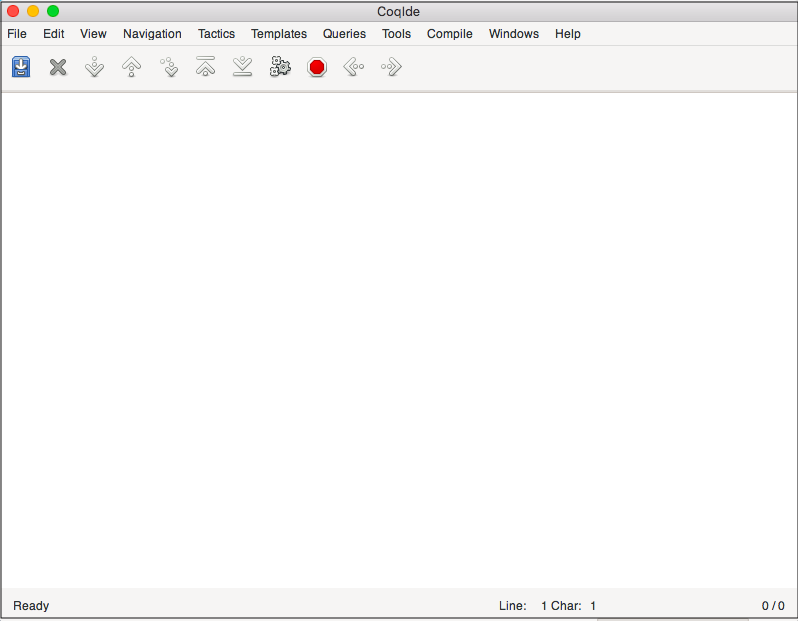
\includegraphics[width=\halfsize]
        		{CoqScreenshots/emptyIDE.png}
	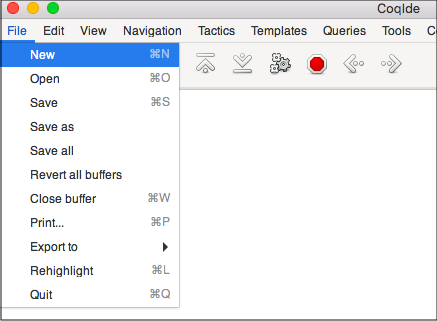
\includegraphics[width=\halfsize]
        		{CoqScreenshots/FixEmptyIDE.png}}
        
        \label{fig: IDEempty} 
        \captionof{figure}{CoqIDE v8.10.2  
        (a) empty IDE screen (b) getting new scratch script buffer open }
\end{minipage}

~\\~\\ 
Go to "File" then "New" to get a new scratch script buffer open if you've accidentally closed out all of your script buffers. Alternately, you can go to "File" then "Open" if you'd like to open a saved file. 


\subsection{Can't close "Load File" Window}

\begin{minipage}{\linewidth}
\center{
	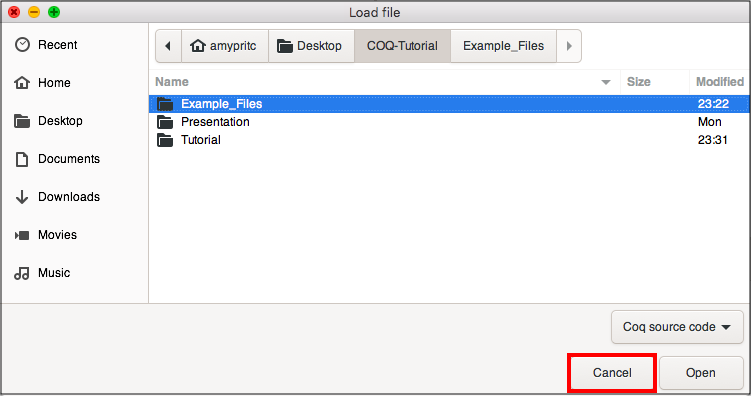
\includegraphics[width=\linewidth]
        		{CoqScreenshots/load_file.png}}
        \label{fig: LoadFile} 
        \captionof{figure}{CoqIDE v8.10.2 Load File window}
\end{minipage}

~\\~\\
If the "Load File" window won't close using the red X in the upper left-hand corner, 
use the "Cancel" button in the lower right (outlined in red). 




